\section{}
\label{sec:p1}
%%%%%%%%%%%%%%%%%%%%%%%%%%%%%%%%%%%%%%%%%%%%%%%%%%%%%%%%%%%%%%%%%%%%%%
\paragraph{a)}
The '\textit{seismic.dat}' data contains seismic data on a regular grid $(75\times75)$, $L_D$, denoted as $\{d(\vect{x}) \ssep \vect{x}\in L_D\} \ssep d(\vect{x})\in \R$, and visually represented by the map in Figure \ref{fig:data}.
The seismic data has the likelihood model given by the equation
\begin{equation}
    [d_i\given\vect{l}] = \begin{cases}
                                0.02 + U_i, & l_i = 0 \Rightarrow \mathrm{sand} \\
                                0.08 + U_i, & l_i = 1 \Rightarrow \mathrm{shale}
                             \end{cases}
                            , i = 1, 2, ..., n,
    \label{eq:likelihood}
\end{equation}

where $U_i \overset{\mathrm{iid}}{\sim}\N\{0,0.06^2\}$. This means that we can rewrite Equation \ref{eq:likelihood} to 
\begin{equation}
    [d_i\given\vect{l}] = \begin{cases}
                                A_i\overset{\mathrm{iid}}{\sim}\N\{0.02,0.06^2\}, & l_i = 0 \Rightarrow \mathrm{sand} \\
                                B_i\overset{\mathrm{iid}}{\sim}\N\{0.08,0.06^2\}, & l_i = 1 \Rightarrow \mathrm{shale}
                             \end{cases}
                            , i = 1, 2, ..., n.
    \label{eq:likelihood2}
\end{equation}
The likelihood model $p(\vect{d}\given \vect{l})$ is then given by 
\begin{equation}
    \begin{array}{rcl}
        [\vect{d}\given\vect{l}] \sim p(\vect{d}\given\vect{l}) & = & \prod\limits_{i=1}^n p(d_i\given l_i) \\
        & = & (0.0072\pi)^{-n/2} \prod\limits_{i=1}^n l_i \exp\left\{\frac{(d_i - 0.08)^2}{0.0072} \right\} + (1-l_i) \exp\left\{\frac{(d_i - 0.02)^2}{0.0072} \right\} \\
         & = & (0.0072\pi)^{-n/2} \exp\left\{\frac{1}{0.0072} \left[\sum\limits_{i \st l_i = 0} (d_i - 0.02)^2 + \sum\limits_{i \st l_i = 1} (d_i - 0.08)^2\right]\right\} \, .
    \end{array}
    \label{eq:likelihood3}
\end{equation}

\begin{figure}
    \centering
    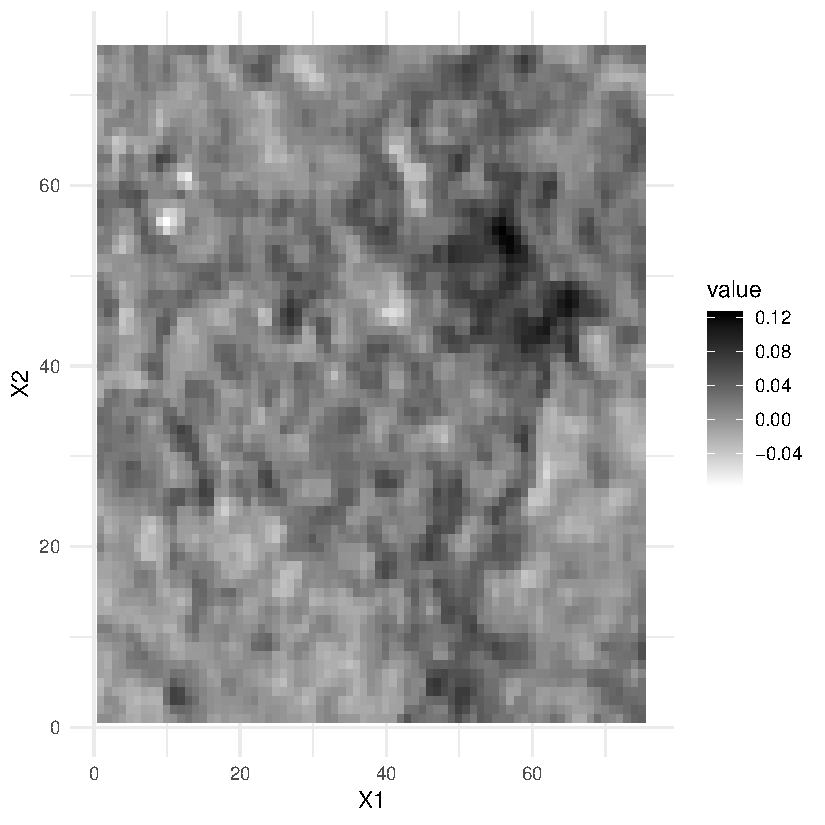
\includegraphics[scale=0.95]{figures/seismic_data.pdf}
    \caption{Map of the seismic data $d(\vect{x})$ on a grid $\matr{L_D}$}
    \label{fig:data}
\end{figure}
%%%%%%%%%%%%%%%%%%%%%%%%%%%%%%%%%%%%%%%%%%%%%%%%%%%%%%%%%%%%%%%%%%%%%%
\paragraph{b)}
We consider a uniform form prior $\prob(\vect{l}) = const$. We have $\prob(\vect{l}) = \prod_{i=1}^n \prob(l_i)$ and $\prob(l_i) = 1/2$. Assuming the data are collected independently, i.e. $\prob(\vect{d}) = \prod_{i=1}^n \prob(d_i)$, we get the posterior
%
\begin{align*}
    \prob(\vect{l} \given \vect{d}) &= \frac{\prob(\vect{d} \given \vect{l}) \prob(\vect{l})}{\prob(\vect{d})} \\
    &= \prod_{i=1}^n \frac{\prob(d_i \given l_i) \prob(l_i)}{\prob(d_i)} \\
    &= \prod_{i=1}^n \prob(l_i \given d_i) \, ,
\end{align*}
%
where $\prob(d_i) = 1/2 \cdot [\prob(d_i \given l_i=0) + \prob(d_i \given l_i=1)]$. Thus the values of $l_i$, $i = 1, \dots, n$ are independent Bernoulli random variables with parameters $p_i = \prob(l_i \given d_i)$. The expectation of the $i$th element is $p_i$ and the variance is $p_i(1-p_i)$. 

\figref{fig:b_sims}, \figref{fig:b_mean} and \figref{fig:b_var} show 10 simulations from the posterior distribution, the posterior mean and the posterior variance, respectively. We see that the mean is high where the measurements are high and low where the measurements are low. The variance is low both where the measurements are high and low, while it is larger in ares where the measurements are not clearly indicating whether the is shale or sand in an area. The posterior mean $\E[\vect{l} | \vect{d}]$ is the probability that an area contains shale (1).

\begin{figure}
    \centering
    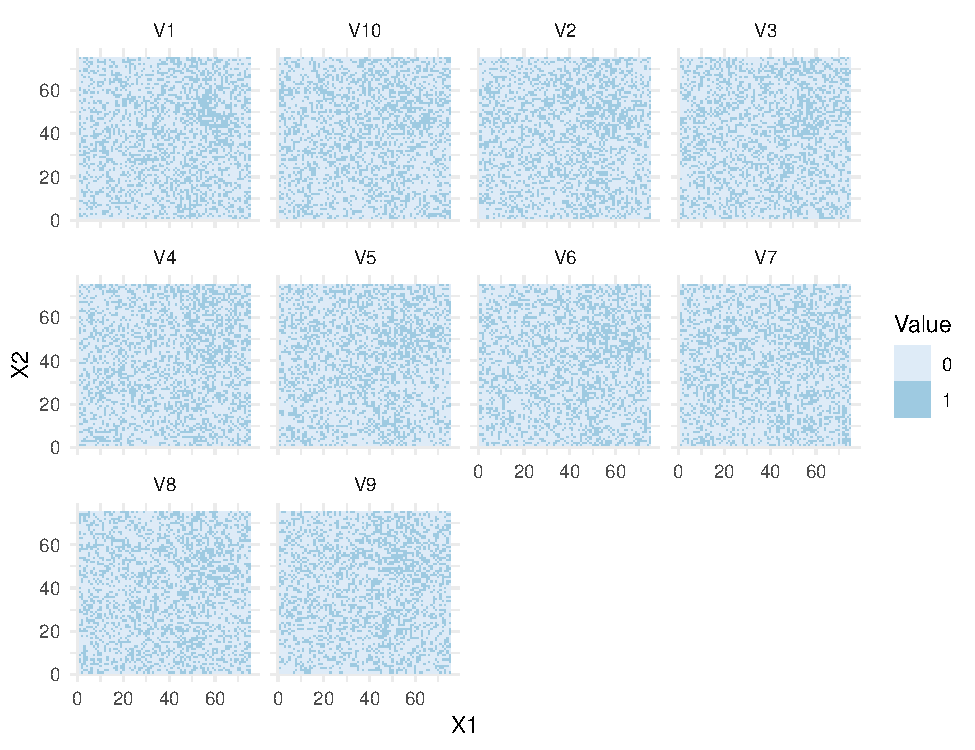
\includegraphics{figures/b_sims.pdf}
    \caption{10 simulations from the posterior given in b).}
    \label{fig:b_sims}
\end{figure}

\begin{figure}
    \centering
    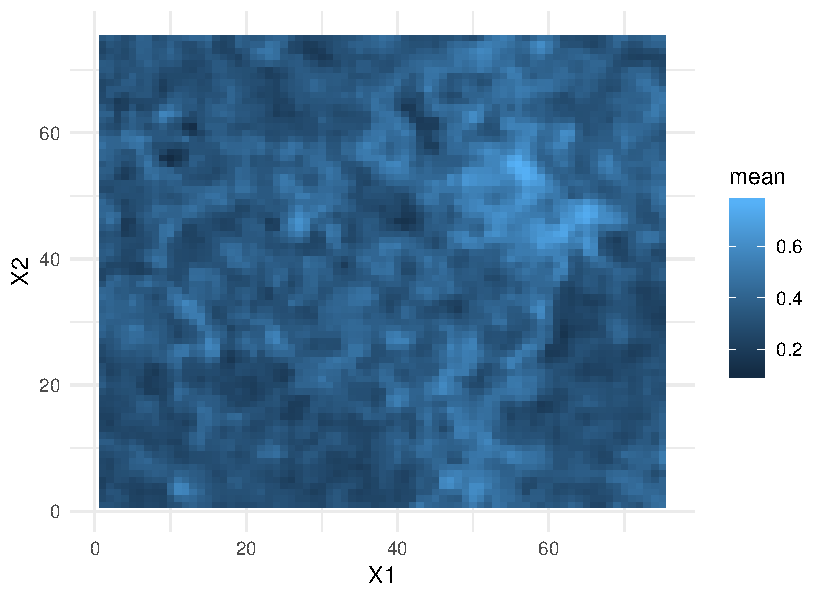
\includegraphics{figures/b_mean.pdf}
    \caption{Posterior mean as derived in b).}
    \label{fig:b_mean}
\end{figure}

\begin{figure}
    \centering
    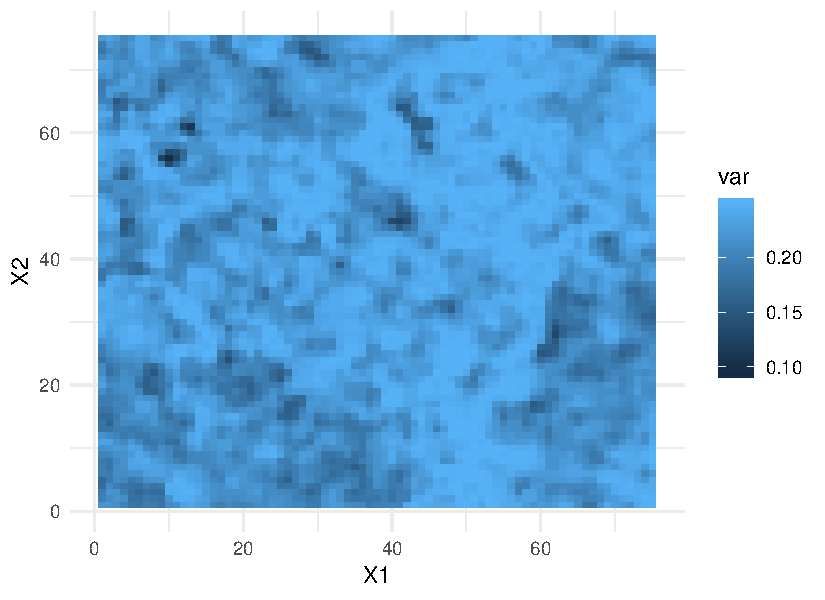
\includegraphics{figures/b_var.pdf}
    \caption{Posterior variance as derived in b).}
    \label{fig:b_var}
\end{figure}

The maximum marginal posterior predictor $\text{MMAP}\left\{\vect{l}|\vect{d}\right\}$ is the vector of values maximizing $p(l_i \given d_i)$, $i = 1, \dots, n$, which are 1 where $p(l_i \given d_i) > 0.5$ and 0 else. A plot of the MMAP is shown in \figref{fig:b_mmap}.

\begin{figure}
    \centering
    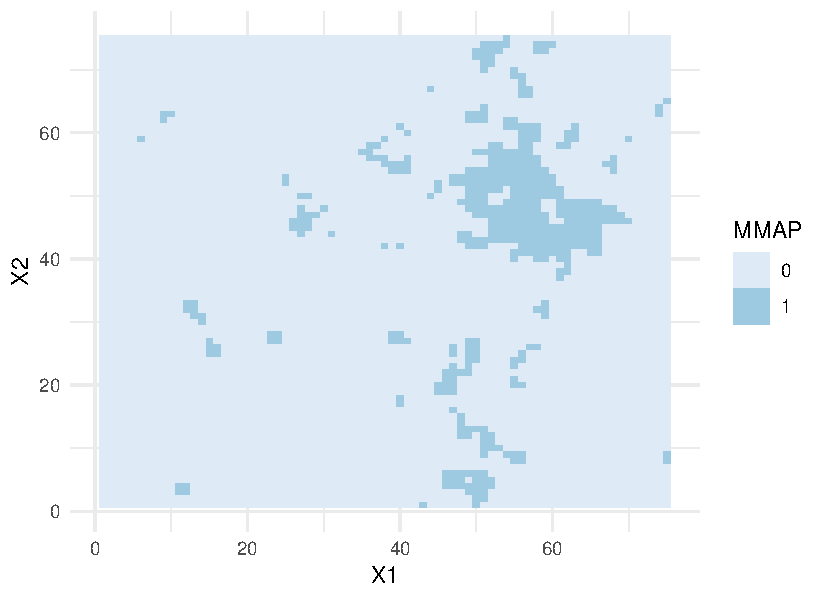
\includegraphics{figures/b_mmap.pdf}
    \caption{Maximum marginal posterior predictor as derived in b).}
    \label{fig:b_mmap}
\end{figure}

%%%%%%%%%%%%%%%%%%%%%%%%%%%%%%%%%%%%%%%%%%%%%%%%%%%%%%%%%%%%%%%%%%%%%%
\paragraph{c)}
We will now consider a Markov RF prior model for $\{l(\vect{x}; \vect{x} \in L_D\}$, represented by the vector $\vect{l}$.
This can be specified by the Markov formulation or Gibbs formulation. The Markov formulation for the prior is 

\begin{equation}
    p(l_i|l_j; j \in \vect{n}_i) = const_M \times \exp{\{\beta \sum_{j\in \vect{n}_i} I(l_i = l_j)\}}; \quad i = 1,2,...n,
\end{equation}
where $\vect{n}_i$ is the neighborhood of grid node $i$, consisting of the four closest grid nodes and $I(.)$ is the indicator function. This is the Ising model. 

This neighboring system corresponds to a clique system where each clique consists of two neighboring nodes, and we write it
\begin{equation}
    \vect{C}_L = \{<i,j>; i,j \in L_D\}
\end{equation}

Then the associated Gibbs formulation of the prior is

\begin{align}
    p(\vect{l}) &= const_G \times \prod_{<i,j>} \exp{\{\beta I(l_i = l_j)\}}\\
    & = const_G \times \exp{\{\beta \sum_{<i,j>} I(l_i = l_j)\}}.
\end{align}

Further, we can find expressions for the posterior distributions $p(\vect{l}|\vect{d})$ and $p(l_i | \vect{d}, \vect{l}_{-i})$, $i = 1, \dots, n$ and index $-i$ meaning all nodes except $i$. 

\begin{align}
\begin{split}
    p(l_i | \vect{d}, \vect{l}_{-i}) &= \frac{p(\vect{d}|\vect{l})p(l_i|\vect{l}_{-i})}{p(\vect{d}|\vect{l}_{-i})}  = \frac{\prod_{k} p(d_k|l_k)\times p(l_i|l_j; j\in \vect{n}_i)}{p(d_i|\vect{l}_{-i})\prod_{k\neq i}p(d_k|l_k)}\\
    & = \frac{p(d_i|l_i)p(l_i|l_j; j\in \vect{n}_i)}{p(d_i|\vect{l}_{-i})},
\end{split}
\label{eq:full_cond}
\end{align}

where $p(d_i|\vect{l}_{-i}) = \sum_{l_i^*\in \{0,1\}} p(d_i|l_i^*)p(l_i^*|l_j; j\in \vect{n}_i)$ and $p(d_i|l_i)$ and $p(l_i|l_j; j\in \vect{n}_i)$ have been specified previously. 

\begin{equation*}
    p(\vect{l}|\vect{d}) = \frac{p(\vect{d}|\vect{l})p(\vect{l})}{p(\vect{d})} = \frac{p(\vect{d}|\vect{l})p(\vect{l})}{\sum_{\vect{l^*}}p(\vect{d}|\vect{l^*})p(\vect{l^*})} ,
\end{equation*}

so that  $p(\vect{d})$ is a sum of all $2^n$ possible configurations of the $n$-vector $\vect{l}$.

The aim is to produce realizations from the posterior distribution $p(\vect{l}|\vect{d})$ and find the posterior mean $\E[\vect{l} | \vect{d}]$, variance $\Var\{\vect{l} | \vect{d}\}$ and alternative prediction $\textrm{MMAP}\{\vect{l} | \vect{d}\}$. We will have to use an MCMC sampler to generate realizations from the posterior, and then $\E[\vect{l} | \vect{d}]$, $\Var\{\vect{l} | \vect{d}\}$ and $\textrm{MMAP}\{\vect{l} | \vect{d}\} = \textrm{argmax}_{l_i}\{ p(l_i|d_i\}$ will be estimated numerically. The latter prediction is calculated simply by counting the frequency of $0$ and $1$ in each position over the posterior realizations, and assigning the one with the highest frequency.

We want to use observations from a comparable domain $D_c \subset \R^2$ to train the prior model, i.e estimate $\beta$. The data from that area is displayed in Figure \ref{fig:complit_data}. Here we have exact observations, and call these $\vect{l}^o$.

\begin{figure}
    \centering
    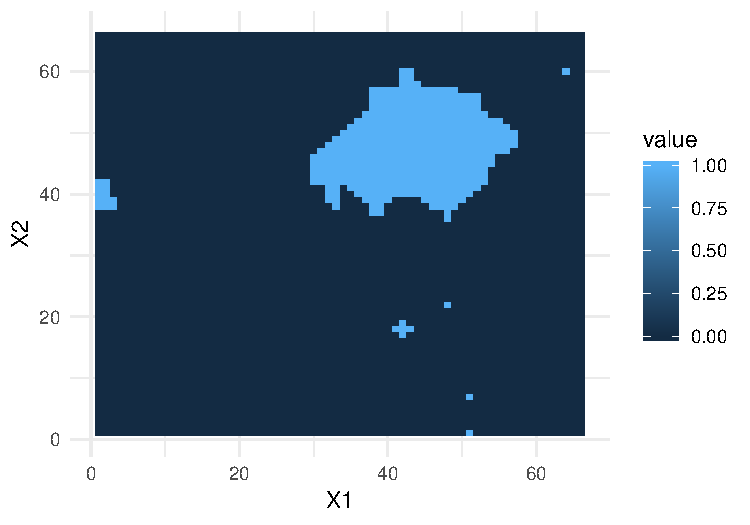
\includegraphics[scale=0.95]{figures/complit_data.pdf}
    \caption{Data from comparable domain $D_c$}
    \label{fig:complit_data}
\end{figure}


We use a maximum psedo-likelihood procedure to estimate $\beta$. We would want to find Maximal Marginal Likelihood (MML) estimate by maximizing $p(\vect{d}; \beta)$, but we have seen that $p(\vect{d})$ is very computer demanding. Thus, we instead maximize the Marginal pseudo-Likelihood (MpL), 

\begin{align*}
     &\prod_{i=1}^n p(d_i, d_j; j \in \vect{n}_i)\\
    &\approx \prod_{i=1}^n \sum_{[l_i^*, l_j^*; j\in \vect{n}_i] \in \{0,1\}} \prod_{j=i, j\in \vect{n}_i} p(d_i|l_i^*)p(l_i^*|l_j^*, j\in \vect{n}_i; \beta)\\
    &:= \hat{p}(\vect{d}; \beta).
\end{align*}
 
Since we have exact observations, this simplifies to 
\begin{equation*}
    \hat{p}(\vect{d}; \beta) = \hat{p}(\vect{l}^o; \beta) = \prod_{i=1}^n p(l_i^o|l_j^o, j\in \vect{n}_i; \beta), 
\end{equation*}

with 
\begin{equation*}
    p(l_i^o|l_j^o, j\in \vect{n}_i; \beta) = \frac{\exp{\{\beta \sum_{j\in \vect{n}_i} I(l_i = l_j)\}}}{\sum_{l_i^*\in \{0,1\}}\exp{\{\beta \sum_{j\in \vect{n}_i} I(l_i^* = l_j)\}}}.
\end{equation*}

Thus, 
\begin{equation*}
    \hat\beta = \textrm{argmax}_{\beta} \{\log(\hat{p}(\vect{l}^o; \beta))\},
\end{equation*}
which we find using the optim() function in R to be $\hat\beta = 1.72$.

We now want to generate realizations from the posterior distribution $p(\vect{l}|\vect{d}; \hat\beta)$. We do this by using MCMC/Gibbs sampler. To avoid boundary problems, we use wrapping boundary conditions, which means that we let the system vertically and horizontally periodic, so that when we need a value that is located outside the grid, we use the value on the other side of the grid, vertically or horizontally.

In the Gibbs sampler, we propose a value (either $0$ or $1$) for one location at a time, from $p(l_i|\vect{d}, \vect{l}_{-i})$ as given in equation \eqref{eq:full_cond}.
Because of the properties of this full conditional distribution, the acceptance probability is always 1, so the step is always accepted. It is obvious that we will have to propose to change quite a few locations before the the chain can converge and between realizations that we can assume are independent. Therefore, realizations of the chain is only saved for every $n = 75 \times 75$ proposals. This will be called one iteration. That is, when we run the MCMC $2000$ iterations, $n\cdot 2000$ locations have been proposed to change.

To assess the question of convergence, we display the fraction of 0 and 1 in the Markov Chain. This is shown in Figure \ref{fig:MCMC_frac}. By this trace plot, it at least seems that the fractions have stabilized. This is of course not a proof of convergence. In particular, it should be noted that it is possible to reach the situation were all tiles become 0 (sand), and it is very hard to get out of this stage. This has not happened in this iteration, and we assume that the chain gives us samples from the posterior distribution after just a short burn-in period. To be sure, we disregard the first $500$ samples.

\begin{figure}
    \centering
    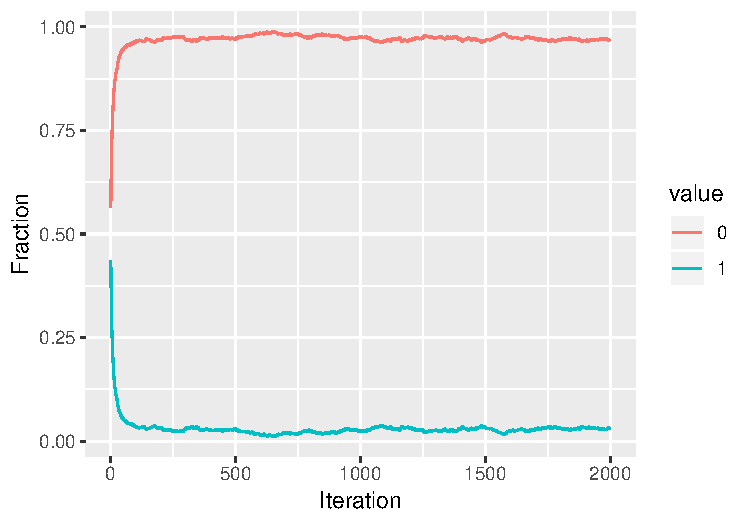
\includegraphics[scale=0.95]{figures/fractionMCMC.pdf}
    \caption{MCMC trace plot of the fraction of grid points with value 0 (sand) and 1 (shale).}
    \label{fig:MCMC_frac}
\end{figure}

In Figure \ref{fig:MCMC_realiz}, 10 realizations of the posterior distribution are shown. These are drawn from the MCMC samples, evenly spaced out between sample 600 and 2000. This means that a lot of changes are proposed between each realization, so that we can assume they are independent. The realizations are similar, but have individual differences, just as we would expect if they are drawn from the same distribution.

\begin{figure}
    \centering
    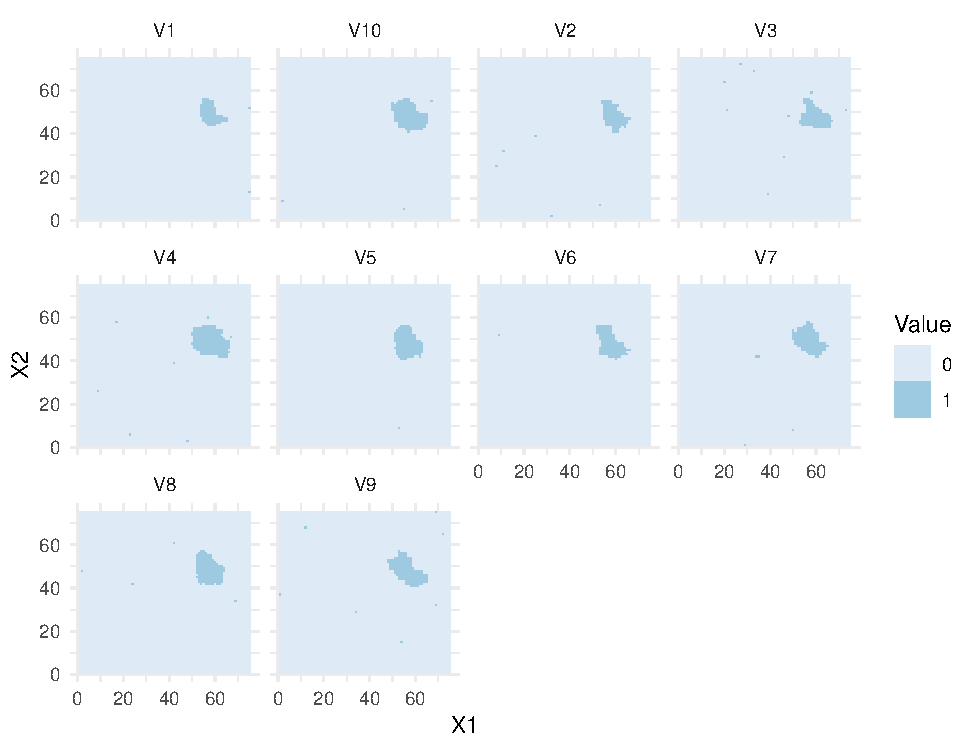
\includegraphics[scale=0.95]{figures/realizations_MCMC.pdf}
    \caption{10 independent realizations from the posterior distribution for the Markov RF, obtained by MCMC.}
    \label{fig:MCMC_realiz}
\end{figure}

We can now compute and plot the posterior mean, variance and MMAP for each grid node. These are displayed in Figures \ref{fig:MCMC_mean}, \ref{fig:MCMC_var} and \ref{fig:MCMC_MMAP}, respectively. We see that in the MMAP, and also indicated in the posterior mean, we get a clear area of shale in the upper right corner ($l_i = 1$), and sand everywhere else. The realizations have the same trend, though the shape of shale area differ somewhat and they get some small areas or single grid points with shale in between the sand. The variance is only somwhat large for a very small area, as the difference in shape is not very large between the realizations. We also observe that the degree of clustering is very similar to the data from the comparable domain $D_c$ displayed in Figure \ref{fig:complit_data}, as this is the data we have used to estimate $\beta$. The posterior distribution is affected by this parameter from the prior model, as well as by the nature of the observed data, shown in Figure \ref{fig:data}.

\begin{figure}
    \centering
    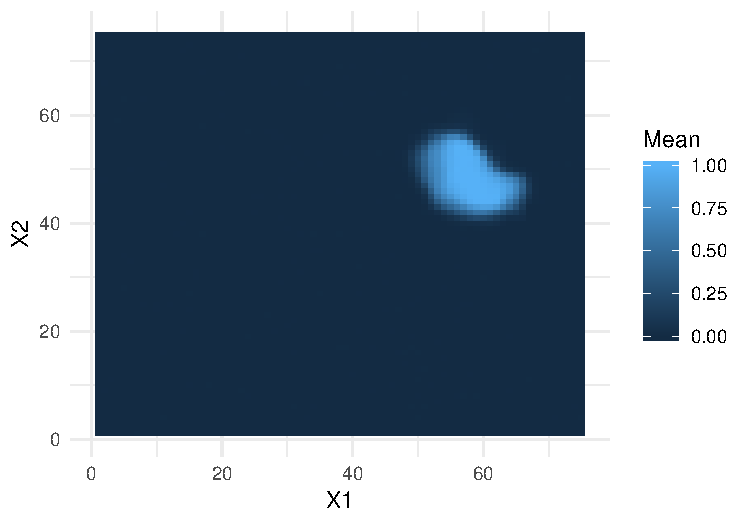
\includegraphics[scale=0.95]{figures/c_mean.pdf}
    \caption{Posterior mean, obtained from a Markov RF prior model using MCMC.}
    \label{fig:MCMC_mean}
\end{figure}

\begin{figure}
    \centering
    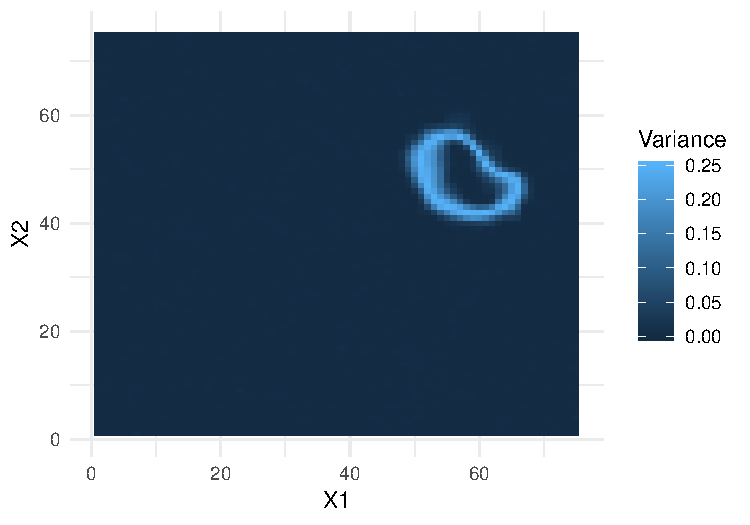
\includegraphics[scale=0.95]{figures/c_variance.pdf}
    \caption{Posterior variance, obtained from a Markov RF prior model using MCMC}
    \label{fig:MCMC_var}
\end{figure}

\begin{figure}
    \centering
    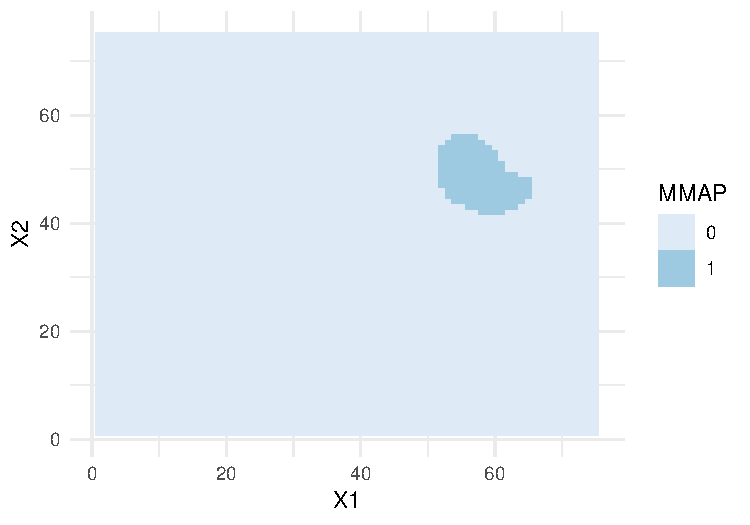
\includegraphics[scale=0.95]{figures/c_MMAP.pdf}
    \caption{Maximum marginal posterior predictor, obtained from a Markov RF prior model using MCMC}
    \label{fig:MCMC_MMAP}
\end{figure}

%%%%%%%%%%%%%%%%%%%%%%%%%%%%%%%%%%%%%%%%%%%%%%%%%%%%%%%%%%%%%%%%%%%%%%
\paragraph{d)}

We see that the results obtained in b) and c) are quite different. In b) we assume independence between the the values $l_i, i= 1,\dots,n$, which means that we get very limited information, and we have a lot of mixing in the posterior realizations. In both cases, we get somewhat more shale ($l_i = 1$) in the upper right corner, just as we have observed the highest values in this corner, but the picture is a lot clearer in c). Here, the values drawn from the posterior are a lot more clustered. This shows that adding a dependency of only the four closest neighbors yields a significant difference.

